% Options for packages loaded elsewhere
\PassOptionsToPackage{unicode}{hyperref}
\PassOptionsToPackage{hyphens}{url}
\PassOptionsToPackage{dvipsnames,svgnames,x11names}{xcolor}
%
\documentclass[
  letterpaper,
  DIV=11,
  numbers=noendperiod]{scrartcl}

\usepackage{amsmath,amssymb}
\usepackage{iftex}
\ifPDFTeX
  \usepackage[T1]{fontenc}
  \usepackage[utf8]{inputenc}
  \usepackage{textcomp} % provide euro and other symbols
\else % if luatex or xetex
  \usepackage{unicode-math}
  \defaultfontfeatures{Scale=MatchLowercase}
  \defaultfontfeatures[\rmfamily]{Ligatures=TeX,Scale=1}
\fi
\usepackage{lmodern}
\ifPDFTeX\else  
    % xetex/luatex font selection
\fi
% Use upquote if available, for straight quotes in verbatim environments
\IfFileExists{upquote.sty}{\usepackage{upquote}}{}
\IfFileExists{microtype.sty}{% use microtype if available
  \usepackage[]{microtype}
  \UseMicrotypeSet[protrusion]{basicmath} % disable protrusion for tt fonts
}{}
\makeatletter
\@ifundefined{KOMAClassName}{% if non-KOMA class
  \IfFileExists{parskip.sty}{%
    \usepackage{parskip}
  }{% else
    \setlength{\parindent}{0pt}
    \setlength{\parskip}{6pt plus 2pt minus 1pt}}
}{% if KOMA class
  \KOMAoptions{parskip=half}}
\makeatother
\usepackage{xcolor}
\setlength{\emergencystretch}{3em} % prevent overfull lines
\setcounter{secnumdepth}{5}
% Make \paragraph and \subparagraph free-standing
\ifx\paragraph\undefined\else
  \let\oldparagraph\paragraph
  \renewcommand{\paragraph}[1]{\oldparagraph{#1}\mbox{}}
\fi
\ifx\subparagraph\undefined\else
  \let\oldsubparagraph\subparagraph
  \renewcommand{\subparagraph}[1]{\oldsubparagraph{#1}\mbox{}}
\fi


\providecommand{\tightlist}{%
  \setlength{\itemsep}{0pt}\setlength{\parskip}{0pt}}\usepackage{longtable,booktabs,array}
\usepackage{calc} % for calculating minipage widths
% Correct order of tables after \paragraph or \subparagraph
\usepackage{etoolbox}
\makeatletter
\patchcmd\longtable{\par}{\if@noskipsec\mbox{}\fi\par}{}{}
\makeatother
% Allow footnotes in longtable head/foot
\IfFileExists{footnotehyper.sty}{\usepackage{footnotehyper}}{\usepackage{footnote}}
\makesavenoteenv{longtable}
\usepackage{graphicx}
\makeatletter
\def\maxwidth{\ifdim\Gin@nat@width>\linewidth\linewidth\else\Gin@nat@width\fi}
\def\maxheight{\ifdim\Gin@nat@height>\textheight\textheight\else\Gin@nat@height\fi}
\makeatother
% Scale images if necessary, so that they will not overflow the page
% margins by default, and it is still possible to overwrite the defaults
% using explicit options in \includegraphics[width, height, ...]{}
\setkeys{Gin}{width=\maxwidth,height=\maxheight,keepaspectratio}
% Set default figure placement to htbp
\makeatletter
\def\fps@figure{htbp}
\makeatother
\newlength{\cslhangindent}
\setlength{\cslhangindent}{1.5em}
\newlength{\csllabelwidth}
\setlength{\csllabelwidth}{3em}
\newlength{\cslentryspacingunit} % times entry-spacing
\setlength{\cslentryspacingunit}{\parskip}
\newenvironment{CSLReferences}[2] % #1 hanging-ident, #2 entry spacing
 {% don't indent paragraphs
  \setlength{\parindent}{0pt}
  % turn on hanging indent if param 1 is 1
  \ifodd #1
  \let\oldpar\par
  \def\par{\hangindent=\cslhangindent\oldpar}
  \fi
  % set entry spacing
  \setlength{\parskip}{#2\cslentryspacingunit}
 }%
 {}
\usepackage{calc}
\newcommand{\CSLBlock}[1]{#1\hfill\break}
\newcommand{\CSLLeftMargin}[1]{\parbox[t]{\csllabelwidth}{#1}}
\newcommand{\CSLRightInline}[1]{\parbox[t]{\linewidth - \csllabelwidth}{#1}\break}
\newcommand{\CSLIndent}[1]{\hspace{\cslhangindent}#1}

\usepackage{booktabs}
\usepackage{longtable}
\usepackage{array}
\usepackage{multirow}
\usepackage{wrapfig}
\usepackage{float}
\usepackage{colortbl}
\usepackage{pdflscape}
\usepackage{tabu}
\usepackage{threeparttable}
\usepackage{threeparttablex}
\usepackage[normalem]{ulem}
\usepackage{makecell}
\usepackage{xcolor}
\usepackage{siunitx}

  \newcolumntype{d}{S[
    input-open-uncertainty=,
    input-close-uncertainty=,
    parse-numbers = false,
    table-align-text-pre=false,
    table-align-text-post=false
  ]}
  
\KOMAoption{captions}{tableheading}
\usepackage{float} \floatplacement{figure}{H}
\makeatletter
\makeatother
\makeatletter
\makeatother
\makeatletter
\@ifpackageloaded{caption}{}{\usepackage{caption}}
\AtBeginDocument{%
\ifdefined\contentsname
  \renewcommand*\contentsname{Table of contents}
\else
  \newcommand\contentsname{Table of contents}
\fi
\ifdefined\listfigurename
  \renewcommand*\listfigurename{List of Figures}
\else
  \newcommand\listfigurename{List of Figures}
\fi
\ifdefined\listtablename
  \renewcommand*\listtablename{List of Tables}
\else
  \newcommand\listtablename{List of Tables}
\fi
\ifdefined\figurename
  \renewcommand*\figurename{Figure}
\else
  \newcommand\figurename{Figure}
\fi
\ifdefined\tablename
  \renewcommand*\tablename{Table}
\else
  \newcommand\tablename{Table}
\fi
}
\@ifpackageloaded{float}{}{\usepackage{float}}
\floatstyle{ruled}
\@ifundefined{c@chapter}{\newfloat{codelisting}{h}{lop}}{\newfloat{codelisting}{h}{lop}[chapter]}
\floatname{codelisting}{Listing}
\newcommand*\listoflistings{\listof{codelisting}{List of Listings}}
\makeatother
\makeatletter
\@ifpackageloaded{caption}{}{\usepackage{caption}}
\@ifpackageloaded{subcaption}{}{\usepackage{subcaption}}
\makeatother
\makeatletter
\@ifpackageloaded{tcolorbox}{}{\usepackage[skins,breakable]{tcolorbox}}
\makeatother
\makeatletter
\@ifundefined{shadecolor}{\definecolor{shadecolor}{rgb}{.97, .97, .97}}
\makeatother
\makeatletter
\makeatother
\makeatletter
\makeatother
\ifLuaTeX
  \usepackage{selnolig}  % disable illegal ligatures
\fi
\IfFileExists{bookmark.sty}{\usepackage{bookmark}}{\usepackage{hyperref}}
\IfFileExists{xurl.sty}{\usepackage{xurl}}{} % add URL line breaks if available
\urlstyle{same} % disable monospaced font for URLs
\hypersetup{
  pdftitle={Physical activity is as tied to obesity as we expect it to be},
  pdfauthor={Victor Ma},
  colorlinks=true,
  linkcolor={blue},
  filecolor={Maroon},
  citecolor={Blue},
  urlcolor={Blue},
  pdfcreator={LaTeX via pandoc}}

\title{Physical activity is as tied to obesity as we expect it to
be\thanks{Code and data are available at:
https://github.com/bestmustard/activity-bmi}}
\usepackage{etoolbox}
\makeatletter
\providecommand{\subtitle}[1]{% add subtitle to \maketitle
  \apptocmd{\@title}{\par {\large #1 \par}}{}{}
}
\makeatother
\subtitle{An analysis of American exerise habits and their BMI}
\author{Victor Ma}
\date{March 16, 2024}

\begin{document}
\maketitle
\ifdefined\Shaded\renewenvironment{Shaded}{\begin{tcolorbox}[boxrule=0pt, sharp corners, enhanced, interior hidden, frame hidden, borderline west={3pt}{0pt}{shadecolor}, breakable]}{\end{tcolorbox}}\fi

\hypertarget{introduction}{%
\section{Introduction}\label{introduction}}

In the context of public health crises, the term `pandemic' comes with
the connotation of infectious diseases sweeping across global
populations. Yet, the United States finds itself grappling with a
pandemic of a different nature, with similarly far-reaching
consequences: obesity. It is no secret that obesity comes with a
multitude of direct health impacts- including increased risk of stroke,
high blood pressure, type 2 diabetes, and even mental health problems
like clinical depression and anxiety ({``Health Effects of Overweight
and Obesity''} 2022). Obesity is recognized as a chronic complex disease
defined by excessive fat deposits that can impair health. In particular,
individuals with a Body Mass Index (BMI) of 30 or above are considered
obese.

America's problem with obesity is long-lasting, with a 30.5\% rate of
obesity observed in the early 2000s (Centers for Disease Control and
Prevention 2021). Marketing companies have taken advantage of this
disease through the spreading of false information, in the form of fad
diets, devices and products tied to fat loss, and misleading nutritional
claims that often prioritize profit over health. In the modern era,
fitness knowledge has been democratized with the advent of social media
and digital platforms aiding in dissemination of health information
(Johnson and Lee 2019). Despite this, obesity in America has only gotten
worse- increasing to 41.9\% in 2020 as one of the top 10 most obese
countries in the world ({``Health Effects of Overweight and Obesity''}
2022).

Obesity is a multifaceted challenge with ties to lifestyle,
socioeconomic factors, and access to health education and resources. In
this study I use a logistic regression model in order to predict the
odds that an individual is obese based on the amount of physical
activity they do per week and their level of income. As logistic
regression models are used to model binary outcomes, my outcome will be
whether an individual has a BMI of 30 or above or not.

The data I am using is from the Center of Disease Control and Prevention
(CDC), a government-officiated service organization dedicated to health
research in the United States. In particular, this dataset contains
information on an adult's diet, physical activity, and weight status
from CDC's Behavioral Risk Factor Surveillance System- America's premier
system for collecting data about health-related risk behaviours
conducted through telephone surveys (Centers for Disease Control and
Prevention (CDC), National Center for Chronic Disease Prevention and
Health Promotion, Division of Nutrition, Physical Activity, and Obesity
2023). I will be focusing on the variables of activity level and level
of income as explanatory variables in the logistic regression model. The
estimand will be the probability that an individual is obese based on
these factors.

My report is structured into four main sections following the
introduction. In the first section, I describe the data utilized for my
analysis, presenting the CDC dataset as well as graphs that show the
distribution of the explanatory variables. The second section details
the logistic regression model, including the rationale for its use and
an interpretation of preliminary findings. Next I will analyse the
variables' impact on obesity prevalence through the use of graphs and
specific numerics from my results. Finally, I discuss the implications
of my findings, address potential weaknesses in my study, and suggest
directions for future research.

This analysis is conducted using R, using several R packages to
facilitate my analysis and presentation. This includes tidyverse for
data manipulation and visualization, knitr for report generation,
modelsummary for model interpretation, and rstanarm for Bayesian
regression modeling (R Core Team 2021; \textbf{Dataverse?}; Xie 2021;
Arel-Bundock 2021; Goodrich et al. 2022; Kay 2021; Wickham et al. 2021).
Some portions including ggplot graphs and the ``Discussion'' section
were written with the help of ChatGPT4 OpenAI (2023). \newpage

\hypertarget{data}{%
\section{Data}\label{data}}

I used a dataset called ``Nutrition, Physical Activity, and Obesity -
Behavioral Risk Factor Surveillance System'' pulled directly from the
CDC website (Centers for Disease Control and Prevention (CDC), National
Center for Chronic Disease Prevention and Health Promotion, Division of
Nutrition, Physical Activity, and Obesity 2023). The .csv file obtained
from the website contains 93250 data points with the relevant
information of an individual's activity level based on their survey
response, BMI, and various demographics. The dataset is owned by the
Division of Nutrition, Physical Activity, Obesity (DNPAO), a division
under the CDC which focuses directly on preventing chronic diseases by
promoting better nutrition practices.

\hypertarget{source-reliability}{%
\subsection{Source Reliability}\label{source-reliability}}

The Centers for Disease Control and Prevention (CDC) is recognized as a
reliable source for obesity data for several reasons. The CDC's Division
of Nutrition, Physical Activity, and Obesity conducts comprehensive
surveillance and research to understand and address obesity, focusing on
policy and environmental strategies to promote healthy eating and active
living. The organization collects data from the largest scale health
survey systems in the United States, including both the Behavioral Risk
Factor Surveillance System (BRFSS) and the National Health and Nutrition
Examination Survey (NHANES) ({``Data \& Statistics \textbar{} Overweight
\& Obesity \textbar{} CDC,''} n.d.; {``Overweight \& Obesity \textbar{}
CDC,''} n.d.).

The BRFSS conducts more than 400,000 interviews annually across the
United States, offering state-level estimates of obesity prevalence
among other health parameters. The large sample size it offers provides
a better understanding of the population when compared to smaller
samples ({``4 Comparison of Data Sources Used to Assess Obesity
Prevalence and Trends,''} n.d.).

\hypertarget{limitations}{%
\subsection{Limitations}\label{limitations}}

The CDC is a reputable government-associated organization but the data
did not come without inherent limitations. As with any telephone survey,
respondents are susceptible to lying which would represent false data
points. In addition, even if respondents believe they are telling the
truth, it is possible that they do not have an accurate measurement of,
for example, their activity level. There is no information available
about the methods used to validate this information on the CDC website.

The data used in this paper does not represent the full dataset, as data
points had to be removed for any missing responses. The previously more
robust dataset with 93250 data points was reduced to 10218 in this
process. The categories available for both the respondent variables do
not allow for some details, as the markers for physical activity were
very specific. Many individuals may not adhere directly to the possible
responses in the survey, and it is impossible to account for individuals
who perform more physiccal activity than the provided options. The
income levels also do not provide a broad perspective, with the maximum
level being \$75,000+. There is no evidence or rationale provided
regarding why these options were chosen.

\hypertarget{variables-of-interest}{%
\subsection{Variables of Interest}\label{variables-of-interest}}

\hypertarget{activity-level}{%
\subsubsection{Activity Level}\label{activity-level}}

Physical activity is a determinant of energy expenditure and is
fundamentally linked to obesity and weight management. Regular physical
activity can significantly reduce the risk of becoming obese by
increasing the number of calories the body uses for energy (Hill and
Peters 2003). Conversely, sedentary lifestyles are closely associated
with obesity due to low energy expenditure. Research has consistently
shown that low physical activity levels are predictive of obesity
development over time. Incorporating various forms of exercise,
including strength training and aerobic activities, can aid in
maintaining a healthy weight and preventing obesity (Sallis and Glanz
2012).

\hypertarget{income}{%
\subsubsection{Income}\label{income}}

Income level is a social determinant of health that influences obesity
rates. Higher income levels often correlate with better access to
healthy foods, recreational facilities, and health services, which can
contribute to lower obesity rates (Pickett and Wilkinson 2005).
Conversely, lower income levels are associated with limited access to
healthy food options, reliance on cheaper, calorie-dense processed
foods, and reduced opportunities for physical activity (Drewnowski and
Specter 2010). This economic disparity creates environments conducive to
obesity development, particularly in communities where affordable
healthy options are scarce. Research indicates that socioeconomic
status, including income, plays a substantial role in the prevalence and
distribution of obesity within populations.

\hypertarget{other-variables}{%
\subsubsection{Other Variables}\label{other-variables}}

While I believed nutrition information would have been a suitable
variable, the options provided in the dataset were only if the
individual had ``No Fruits'' or ``No Vegetables'' in their regular diet.
I did not think these two options were enough to make relevant
conclusions.

\hypertarget{data-preparation-and-cleaning}{%
\subsection{Data Preparation and
Cleaning}\label{data-preparation-and-cleaning}}

The data was first downloaded as a .csv file directly from the CDC
website and then saved in parquet format using the arrow package for
efficient storage and access (Richardson et al. 2024). The cleaning
process involved filtering for the columns for the relevant variables
which were ``Topic'' (``Physical Activity - Behavior'', ``Obesity /
Weight Status'', ``Fruits and Vegetables - Behavior''), ``Question''
(specific responses under the topic), BMI, and Income.

The respondent variable of activity level was transformed for
simplicity. Initially, the possible values included: ``Percent of adults
who engage in no leisure-time physical activity'', ``Percent of adults
who engage in muscle-strengthening activities on 2 or more days a
week'', ``Percent of adults who achieve at least 150 minutes a week of
moderate-intensity aerobic physical activity or 75 minutes a week of
vigorous-intensity aerobic activity (or an equivalent
combination)''\ldots{} and so on. I removed the specifics and labelled
them ``No Activity'', ``Strength'', ``Cardio'', ``Cardio + Strength'',
``Double Cardio'', as the markers of strength or cardio training
remained the same throughout (strength meant 2 days of strength
training, cardio meant 150 minutes of moderate intensity or 75 minutes
of ``vigorous-intensity''). ``Double Cardio'' was named as such since it
was defined as double the minutes of cardio as ``Cardio''.

``NA'' responses were then filtered out in order to make sure each data
point contained all the variables used.

The cleaned dataset was then saved in both CSV and parquet formats.

The distributions for each explanatory variable are illustrated in
Figure~\ref{fig-activity} and Figure~\ref{fig-income} below:

\begin{figure}

{\centering 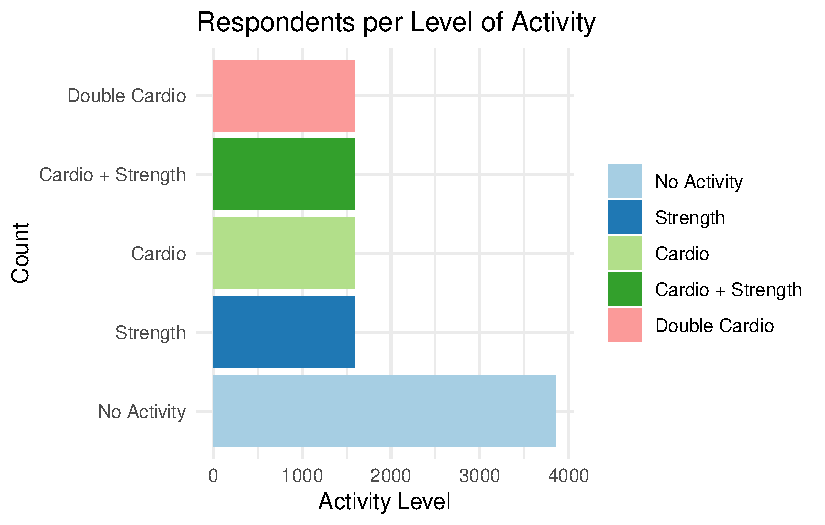
\includegraphics[width=\textwidth,height=0.2\textheight]{paper_files/figure-pdf/fig-activity-1.pdf}

}

\caption{\label{fig-activity}Number of respondents at each activity
level}

\end{figure}

\begin{figure}

{\centering 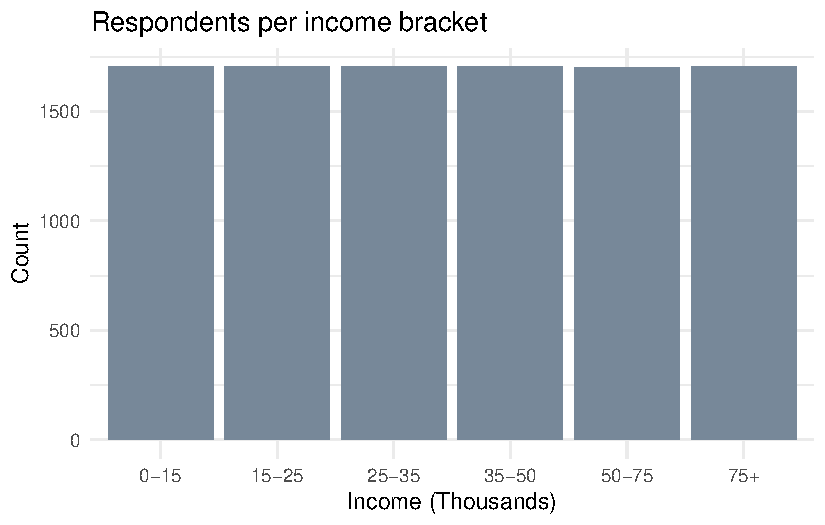
\includegraphics[width=\textwidth,height=0.2\textheight]{paper_files/figure-pdf/fig-income-1.pdf}

}

\caption{\label{fig-income}Number of respondents per income bracket}

\end{figure}

Figure~\ref{fig-activity} tells us that 4-year degree graduates are the
most well represented in the polls, followed by high school graduates,
people with some college, and then 2-year degree graduates. People who
have not graduated high school are hardly represented at all.

In Figure~\ref{fig-income} we see 45-64 being the most dominant age
group, with much less representation in the 18-29 range. Also, about
20\% more females participated in the study than males.

Below are some figures representing who people voted for based on their
age and gender, followed by education level and gender.

\begin{figure}

{\centering 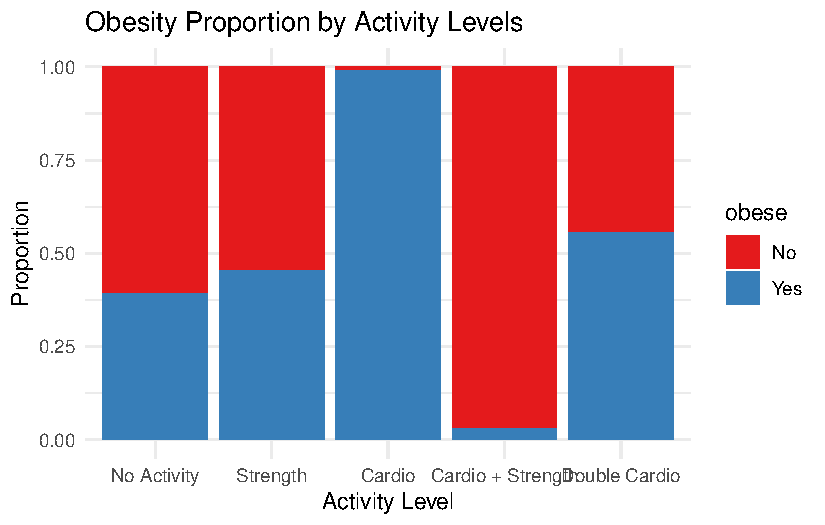
\includegraphics[width=\textwidth,height=0.2\textheight]{paper_files/figure-pdf/fig-activityobesity-1.pdf}

}

\caption{\label{fig-activityobesity}Prevalence of obesity by activity
level}

\end{figure}

Figure~\ref{fig-activityobesity} shows a negative correlation between
votes for Joe Biden and older age groups.

\begin{figure}

{\centering 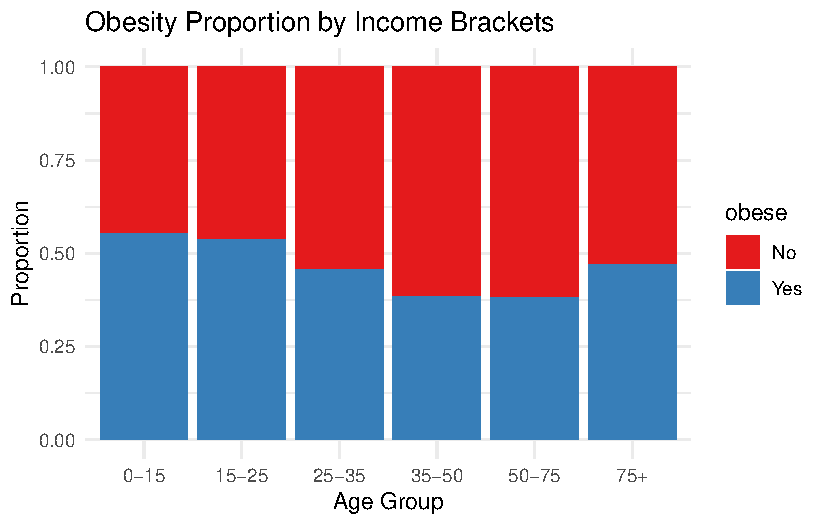
\includegraphics[width=\textwidth,height=0.2\textheight]{paper_files/figure-pdf/fig-incomeobesity-1.pdf}

}

\caption{\label{fig-incomeobesity}Prevalence of obesity by income level}

\end{figure}

We can see that in \textbf{?@fig-gendervotes}, more women voted for Joe
Biden than men.

\hypertarget{model}{%
\section{Model}\label{model}}

Logistic regression is a model used when the outcome or dependent
variable is binary, which fits this scenario perfectly as I am modelling
the binary outcome of below 30 BMI or a BMI of 30 and above.

The regression model will calculate the log odds of the probability that
a person has a BMI of 30 or above, and then map it to a probability
between 0 and 1 through the logistic function.

The standard logistic function \(\sigma(t)\) for a real-valued input
\(t\) is defined as:

\[ \sigma(t) = \frac{1}{1 + e^{-t}} \]

The graph of the logistic function is an S-shaped curve known as a
sigmoid curve. It approaches 1 as \(t\) goes to positive infinity and
approaches 0 as \(t\) goes to negative infinity.

In logistic regression, the input \(t\) is the linear combination of
predictors including the intercept, which can be represented as
\(\beta_0 + \beta_1X_1 + \beta_2X_2 + ... + \beta_nX_n\). The logistic
function then translates this into a probability that the dependent
variable is 1 (has a BMI above 30).

In this situation, I will be using the predictors activity level and
income and then applying the logistic function to get the probability
\(P(Y_i=1)\) that a respondent \(i\) is considered obese.

This model is particularly strong at handling categorical dependent
variables, which each of my explanatory variables fall under (Jr.,
Lemeshow, and Sturdivant 2013).

\hypertarget{model-specification}{%
\subsection{Model Specification}\label{model-specification}}

The logistic regression model is defined as:

\[
\log\left(\frac{P(Y_i=1)}{1 - P(Y_i=1)}\right) = \beta_0 + \beta_1X_{\text{activity},i} + \beta_2X_{\text{income},i}
\]

\hypertarget{model-set-up}{%
\subsection{Model set-up}\label{model-set-up}}

\begin{itemize}
\tightlist
\item
  \(Y_i\) is the binary indicator of having a BMI of 30 or above (1)
  versus a BMI below 30 for respondent \(i\).
\item
  \(X_{\text{activity},i}\), \(X_{\text{income},i}\) are the activity
  level and income of respondent \(i\), respectively.
\item
  \(\beta_0\) represents the model intercept, while \(\beta_1\) and
  \(\beta_2\) are coefficients quantifying the effects of activity level
  and income on the likelihood of being considered obese.
\end{itemize}

I fit my logistic regression model to the data using `stan\_glm()'
function from the `rstanarm' package in R Goodrich et al. (2022). This
function will automatically determine each of the \(\beta\) coefficients
in the model, using a smaller slice sample of 3000 from the data we
processed. This function also uses Bayesian logistic regression with the
default priors from `rstanarm'.

\hypertarget{model-justification}{%
\subsubsection{Model Justification}\label{model-justification}}

After creating the model, we can examine the summary in
Figure~\ref{fig-summary}:

\begin{figure}

{\centering 

\hypertarget{fig-summary-1}{}
\begin{table}
\centering
\begin{tabular}[t]{lc}
\toprule
  & (1)\\
\midrule
(Intercept) & \num{0.060}\\
activityStrength & \num{0.176}\\
activityCardio & \num{5.373}\\
activityCardio + Strength & \num{-2.902}\\
activityDouble Cardio & \num{0.746}\\
income15-25 & \num{0.100}\\
income25-35 & \num{-0.717}\\
income35-50 & \num{-0.984}\\
income50-75 & \num{-1.058}\\
income75+ & \num{-0.396}\\
\midrule
Num.Obs. & \num{3000}\\
R2 & \num{0.340}\\
Log.Lik. & \num{-1435.801}\\
ELPD & \num{-1445.9}\\
ELPD s.e. & \num{25.8}\\
LOOIC & \num{2891.9}\\
LOOIC s.e. & \num{51.6}\\
WAIC & \num{2891.9}\\
RMSE & \num{0.40}\\
\bottomrule
\end{tabular}
\end{table}

}

\caption{\label{fig-summary}Model summary}

\end{figure}

In order to better interpret the results of the model, I can create a
coefficient plot to visually see the effect sizes of the predictor
variables on the likelihood of an individual supporting Biden.

Figure~\ref{fig-coefficient} maps each predictor variable on the y-axis
to an effect size and confidence interval on the x-axis. The effect size
is the change in log-odds of supporting Biden for a one-unit increase in
the predictor variable, which is essentially how much impact each
demographic characterstic has an effect on voting for Biden.

The confidence intervals tell us the range within we can be confident
that the true effect lies. Smaller confidence intervals means there is a
higher level of precision in the estimate of the effect size. I am not
as interested in the intervals that cross zero because that means that
there is data to support each side (Biden or Trump) and so they are less
statistically significant.

\begin{verbatim}
[1] "term"      "estimate"  "std.error"
\end{verbatim}

\begin{figure}

{\centering 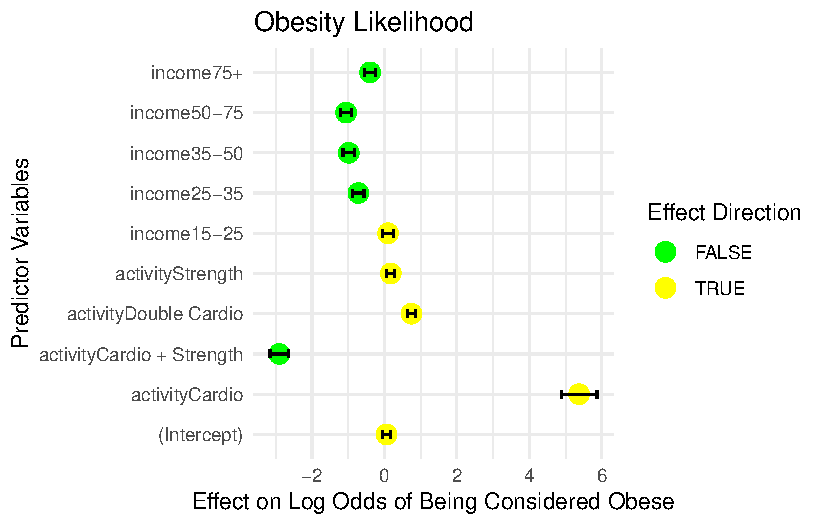
\includegraphics{paper_files/figure-pdf/fig-coefficient-1.pdf}

}

\caption{\label{fig-coefficient}Coefficient plot of demographics}

\end{figure}

The conclusions I can draw from Figure~\ref{fig-coefficient} align with
what I expected given the dataset. It's clear that higher education
levels, specifically 4-year degrees and post-grad degrees, are
positively associated with support for Biden. Higher age groups,
specifically 45-64 and 65+, are strongly tied to voting for Trump. Men
are less likely to vote for Biden than Women.

\newpage

\hypertarget{results}{%
\section{Results}\label{results}}

Figures \textbf{?@fig-page}, \textbf{?@fig-pgender}, and
\textbf{?@fig-pedu} are recreations of the earlier graphs we saw
showcasing the proportion of voters for Joe Biden by groups within each
demographic, where the bar is the data from CCES 2020 while the point is
the prediction generated by the model.

\begin{figure}

{\centering 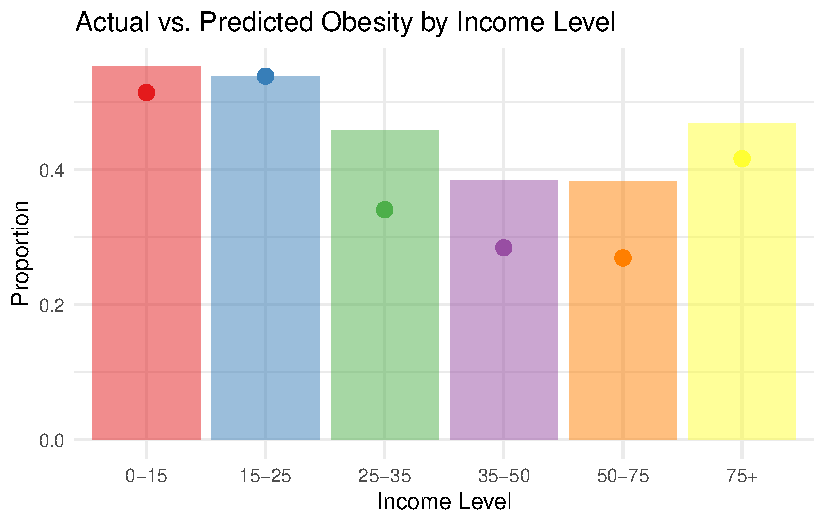
\includegraphics[width=\textwidth,height=0.25\textheight]{paper_files/figure-pdf/fig-pactivity-1.pdf}

}

\caption{\label{fig-pactivity}Model prediction for obesity by income
level vs.~CDC data}

\end{figure}

\begin{figure}

{\centering 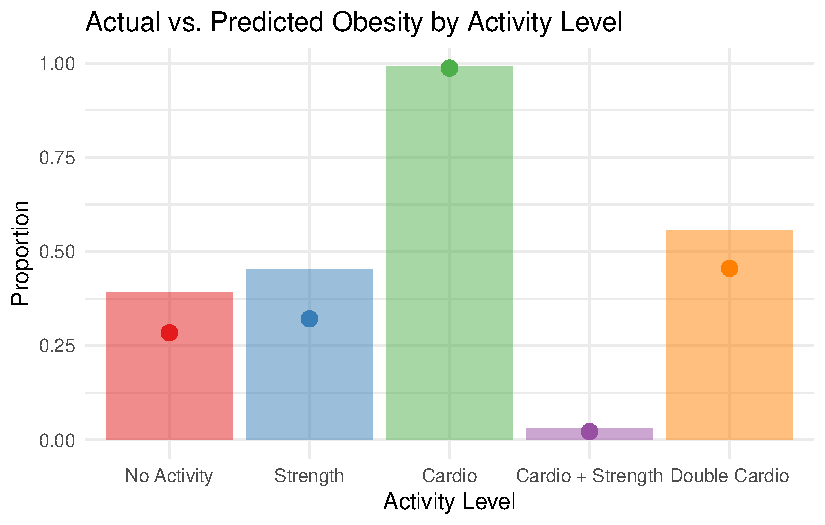
\includegraphics[width=\textwidth,height=0.25\textheight]{paper_files/figure-pdf/fig-pobesity-1.pdf}

}

\caption{\label{fig-pobesity}Model prediction for obesity by activity
level vs.~CDC data}

\end{figure}

By observation, it is evident that the model's prediction was fairly
close to what the CCES data showed. The trend remains the same for each
result. However, gender and education were predicted to have a higher
sentiment of voting for Joe Biden while age had a lower sentiment.

It is worth nothing though that in Figure~\ref{fig-pactivity}, all age
categories showed polling data of above 50\% to vote for Biden. Now with
the lower average vote, the older age categories of ``45-64'' and
``65+'' are leaning towards Trump. On Figure~\ref{fig-pobesity} for the
lower education groups, the ``No-HS'' group which was at just about 50\%
is now above it, and the ``High School Graduate'' is also closer to
voting for Biden. While this may seem marginal, close elections where
voter sentiment is close to 50\% would be largely impacted by changes
like this. Although ultimately this is not an accurate predictor for who
would win the election, only which groups would vote for who.

\hypertarget{discussion}{%
\section{Discussion}\label{discussion}}

\hypertarget{weaknesses-and-next-steps}{%
\section{Weaknesses and Next Steps}\label{weaknesses-and-next-steps}}

\newpage

\hypertarget{references}{%
\section*{References}\label{references}}
\addcontentsline{toc}{section}{References}

\hypertarget{refs}{}
\begin{CSLReferences}{1}{0}
\leavevmode\vadjust pre{\hypertarget{ref-brfss}{}}%
{``4 Comparison of Data Sources Used to Assess Obesity Prevalence and
Trends.''} n.d. The National Academies of Sciences, Engineering,;
Medicine; \url{https://nap.nationalacademies.org/read/23505/chapter/7}.

\leavevmode\vadjust pre{\hypertarget{ref-Modelsummary}{}}%
Arel-Bundock, Vincent. 2021. \emph{Modelsummary: Summary Tables and
Plots for Statistical Models and Data: Beautiful, Customizable, and
Publication-Ready}.
\url{https://CRAN.R-project.org/package=modelsummary}.

\leavevmode\vadjust pre{\hypertarget{ref-obesityfacts}{}}%
Centers for Disease Control and Prevention. 2021. {``Adult Obesity
Facts.''}

\leavevmode\vadjust pre{\hypertarget{ref-dataset}{}}%
Centers for Disease Control and Prevention (CDC), National Center for
Chronic Disease Prevention and Health Promotion, Division of Nutrition,
Physical Activity, and Obesity. 2023. {``{Nutrition, Physical Activity,
and Obesity - Behavioral Risk Factor Surveillance System}.''} Atlanta,
Georgia:
\url{https://chronicdata.cdc.gov/Nutrition-Physical-Activity-and-Obesity/Nutrition-Physical-Activity-and-Obesity-Behavioral/hn4x-zwk7};
{Centers for Disease Control and Prevention}.

\leavevmode\vadjust pre{\hypertarget{ref-cdcdata}{}}%
{``Data \& Statistics \textbar{} Overweight \& Obesity \textbar{}
CDC.''} n.d. Centers for Disease Control; Prevention;
\url{https://www.cdc.gov/obesity/data/index.html}.

\leavevmode\vadjust pre{\hypertarget{ref-drewnowski}{}}%
Drewnowski, Adam, and S. E. Specter. 2010. {``Obesity and the Food
Environment: Dietary Energy Density and Diet Costs.''} \emph{American
Journal of Preventive Medicine} 27: 154--62.

\leavevmode\vadjust pre{\hypertarget{ref-Rstanarm}{}}%
Goodrich, Ben, Jonah Gabry, Imad Ali, and Sam Brilleman. 2022.
{``Rstanarm: {Bayesian} Applied Regression Modeling via {Stan}.''}
\url{https://mc-stan.org/rstanarm/}.

\leavevmode\vadjust pre{\hypertarget{ref-cdc}{}}%
{``Health Effects of Overweight and Obesity.''} 2022. Centers for
Disease Control; Prevention;
\url{https://www.cdc.gov/healthyweight/effects/index.html}.

\leavevmode\vadjust pre{\hypertarget{ref-hillenergy}{}}%
Hill, James O., and John C. Peters. 2003. {``Energy Balance and
Obesity.''} \emph{Circulation} 104: 51--52.

\leavevmode\vadjust pre{\hypertarget{ref-Johnson2019}{}}%
Johnson, Mark K., and Angela R. Lee. 2019. {``The Role of Digital Media
in Shaping Health Behaviors: Opportunities and Challenges.''}
\emph{Health Communication Today} 24 (5): 456--67.

\leavevmode\vadjust pre{\hypertarget{ref-Hosmer2013}{}}%
Jr., David W. Hosmer, Stanley Lemeshow, and Rodney X. Sturdivant. 2013.
\emph{Applied Logistic Regression}. 3rd ed. New York: John Wiley \&
Sons.

\leavevmode\vadjust pre{\hypertarget{ref-Tidybayes}{}}%
Kay, Matthew. 2021. \emph{Tidybayes: Tidy Data and Geoms for Bayesian
Models}. \url{https://CRAN.R-project.org/package=tidybayes}.

\leavevmode\vadjust pre{\hypertarget{ref-chatgpt}{}}%
OpenAI. 2023. {``ChatGPT: Optimizing Language Models for Dialogue.''}
\url{https://openai.com/}.

\leavevmode\vadjust pre{\hypertarget{ref-cdcinitiatives}{}}%
{``Overweight \& Obesity \textbar{} CDC.''} n.d. Centers for Disease
Control; Prevention; \url{https://www.cdc.gov/obesity/index.html}.

\leavevmode\vadjust pre{\hypertarget{ref-pickett}{}}%
Pickett, Kate E., and Richard G. Wilkinson. 2005. {``The Social
Determinants of Health: The Solid Facts.''} \emph{International Journal
of Epidemiology} 34: 1245.

\leavevmode\vadjust pre{\hypertarget{ref-citeR}{}}%
R Core Team. 2021. \emph{R: A Language and Environment for Statistical
Computing}. Vienna, Austria: R Foundation for Statistical Computing.
\url{https://www.R-project.org/}.

\leavevmode\vadjust pre{\hypertarget{ref-arrow}{}}%
Richardson, Neal, Ian Cook, Nic Crane, Dewey Dunnington, Romain
François, Jonathan Keane, Dragoș Moldovan-Grünfeld, Jeroen Ooms, Jacob
Wujciak-Jens, and Apache Arrow. 2024. \emph{Arrow: Integration to
'Apache' 'Arrow'}. \url{https://github.com/apache/arrow/}.

\leavevmode\vadjust pre{\hypertarget{ref-sallisobesity}{}}%
Sallis, James F., and Karen Glanz. 2012. {``Role of Physical Activity in
the Prevention of Obesity in Children.''} \emph{International Journal of
Obesity} 14: 34--38.

\leavevmode\vadjust pre{\hypertarget{ref-Dplyr}{}}%
Wickham, Hadley, Romain François, Lionel Henry, and Kirill Müller. 2021.
\emph{Dplyr: A Grammar of Data Manipulation}.
\url{https://CRAN.R-project.org/package=dplyr}.

\leavevmode\vadjust pre{\hypertarget{ref-Knitr}{}}%
Xie, Yihui. 2021. \emph{Knitr: A General-Purpose Package for Dynamic
Report Generation in r}. \url{https://CRAN.R-project.org/package=knitr}.

\end{CSLReferences}



\end{document}
